\section{System design pattern}

After specifying the requirements and modeling them into use-case and activity diagrams, we will choose and analyze a suitable design pattern for our system. The proposed design pattern is a combination of Layered, Client-Server, and Repository design patterns.

\begin{figure}[H]
    \centering
    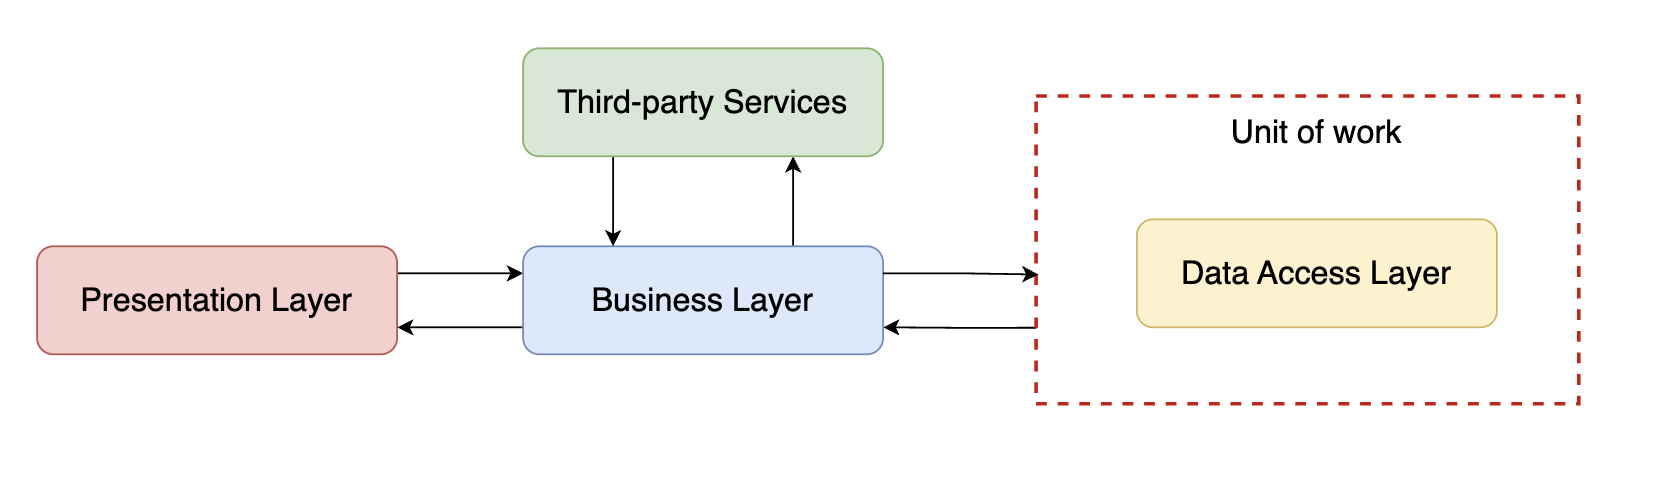
\includegraphics[width=0.8\textwidth]{Figures/design_pattern.png}
    \caption{System design pattern}
\end{figure}

Our system, as a layered application, will be structured into three distinct abstraction layers as shown in Figure 33:


\begin{itemize}
    \item
          \emph{Presentation Layer}: This layer encompasses the UI/UX components that users interact with. It communicates with the Business Layer, managing user events, requesting data, and presenting it to the user.
    \item
          \emph{Business Layer}: This layer executes the core functionality and business flows of the system. It is also tasked with interacting with third-party services.
    \item
          \emph{Data Access Layer}: This layer offers an abstract API to the Business Layer and manages all operations related to database system interaction, such as querying, adding, deleting, or updating data.
\end{itemize}

As for the Client-Server pattern, the Presentation layer is implemented on the client side (Frontend), and the other two layers are implemented on the server side (Backend). Client and Server will interact with each other through a controller layer (web API).

By applying the Repository design pattern, the system has an additional layer that isolates the Data access layer from the Business layer, called “Unit of work”. This layered assembles all the classes in the Data access layer as a single class that encapsulates the logic to access data resources.

\subsubsection*{Advantages of the proposed design pattern}

The Layered design pattern is a straightforward concept to grasp and implement. This pattern offers the advantage of change isolation, meaning that any modifications are confined to the specific layer being altered. This leads to a clear distinction between different types of components and facilitates the consolidation of similar codes in one place. 

Moreover, the separation of the Presentation layer from other layers (due to the Client-Server pattern) paves the way for future mobile application development. This is possible through the reuse of existing functionalities in the Business layer and Data access layer. Thus, the Layered design pattern not only simplifies the learning and implementation process but also enhances adaptability to changes and future developments.

The Repository layer allows us to manage all database access in an isolated manner. It centralizes common data access functionalities, thereby reducing the development effort and enhancing maintainability. This layer serves as a unified platform for all database interactions, streamlining the development process and ensuring easier maintenance.

